\documentclass{standalone}

\usepackage{tikz}

\usetikzlibrary{positioning, chains, shapes.geometric, fit, shapes, arrows.meta, calc}

\begin{document}

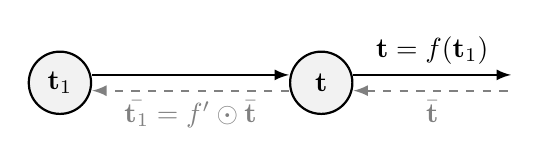
\begin{tikzpicture}[
    >=LaTeX, % Use default LaTeX arrows
    % Styles 
    node/.style={ % Input or output node
        circle,
        minimum width=2.25em,
        draw,
        fill=gray!10,
        thick
    },
    arrow/.style={
        -latex,
        thick
    },
    backprop/.style={ % Backpropagation arrows
        arrow,
        dashed,
        gray
    }
]
    % Computational graph nodes
    \node[node] (t1) {$\mathbf{t}_1$};
    \node[node] (t) [right=of t1, xshift=1.5cm] {$\mathbf{t}$};

    % Computational graph edges
    \draw[arrow] ([yshift=0.1cm]t1.east) -- ([yshift=0.1cm]t.west);
    \draw[arrow] (t.east) +(0cm,0.1cm) -- +(2cm,0.1cm) node[midway, above] {$\mathbf{t} = f(\mathbf{t}_1)$};

    % Backpropagation arrows with partial derivatives
    \draw[backprop, latex-] (t.east) +(0cm,-0.1cm) -- +(2cm,-0.1cm) node[midway, below] {$\bar{\mathbf{t}}$};
    \draw[backprop] ([yshift=-0.1cm]t.west) -- ([yshift=-0.1cm]t1.east) node[midway, below] {$\bar{\mathbf{t}_1} = f' \odot \bar{\mathbf{t}}$};
\end{tikzpicture}

\end{document}